\section{Results and Analysis}

\subsection{The Arrow}

To perform the experiments, we chose to use a paper airplane model called ``The Arrow". See Figure~\ref{fig:arrow} for a picture of The Arrow. 
We chose The Arrow because it required easy construction and had a rigid structure. Due to The Arrow's relatively small wing aspect ratio, it experiences minimal 
flapping motion during flight. As a result, the actual flight condition better resembles what is assumed in the theory. We also applied 
double-sided tape in the middle section to improve its rigidity. We constructed three The Arrows in order to reduce any model-specific
errors, and all experimental results came from an average of these three models. See Figure~\ref{fig:arrowdimension} for the detailed dimension measurements of the three models we used. 

\begin{figure}[hl]
  \centering
    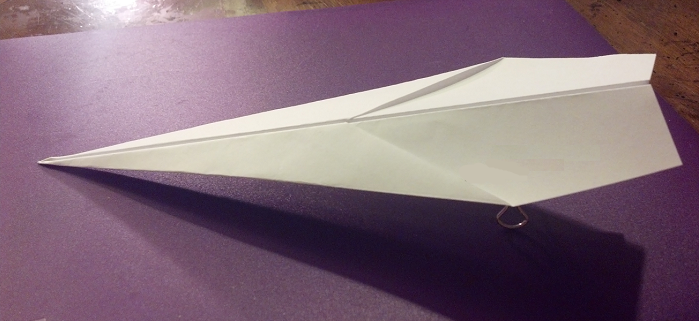
\includegraphics[scale=0.6]{figures/arrow.png}
    \caption{A picture of The Arrow. It is one of the most common paper airplane models. It has a long flight range and 
		         is easy to construct.}
  \label{fig:arrow}
\end{figure}


 
\begin{figure}[hl]
  \centering
    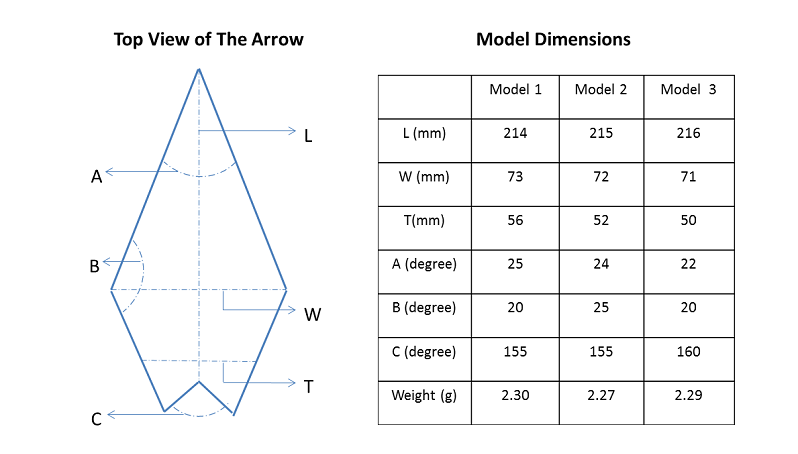
\includegraphics[scale=0.6]{figures/arrowdimension.png}
    \caption{Dimension of The Arrow used in the experiments. The measurements apply to all three models constructed.}
  \label{fig:arrowdimension}
\end{figure}

We launched the paper airplanes manually, and used an iPhone application to record the launching acceleration (see appendix for the source code). To maintain consistency during launch, the paper airplane started right above the launcher's shoulder and was released when the launcher's arm was fully extended. The launching height was measured to be 146cm and the launching distance was measured to be 60cm. Knowing the launching distance and acceleration, we could calculate the releasing speed using the following two simple mechanics equations:

\begin{equation}
	\label{kinematics1}
		d = 1/2 a t^2
\end{equation}

\begin{equation}
	\label{kinematics2}
		v = a t
\end{equation}		

	
\subsection{Stability vs Center of Gravity}
We attached a metal clip of 2.9g to various positions in the middle section of the paper airplanes in order to shift its center of gravity (see Figure~\ref{fig:clip}).


\begin{figure}[hl]
	\centering
		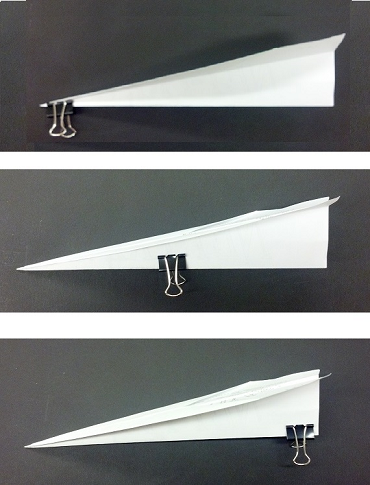
\includegraphics[scale=0.5]{figures/clip.png}
		\caption{We attached a clip of 2.9g to various positions of the paper airplane to shift its center of gravity.}
	\label{fig:clip}
\end{figure}

We then launched The Arrow in the manner described in section 4.1. To measure its stability, we counted the number of rotations the model had completed in the air and the distance it had traveled when landed. A stable flight should have a long travel distance and minimal rotations.
Figure~\ref{fig:centerofgravity} shows the experimental result. 


\begin{figure}[hl]
	\centering
		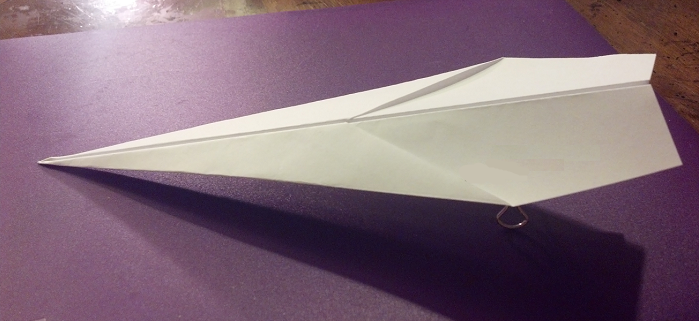
\includegraphics[scale=0.5]{figures/centerofgravity.png}
		\caption{Flight stability v.s. the center of gravity. The flight distance and number of ratations in the air provide a qualitative measure of the flight 
		stability: the longer the distance and fewer ratations, the more stable the flight.}
	\label{fig:centerofgravity}
\end{figure}

According to section XXX, the aerodynamic center is at a quarter length from the front of the aerofoil. Center of gravity before this point gives a stable flight, and
after this point produces a turbulent flight. This is demonstrated qualitatively by Figure~\ref{fig:centerofgravity}. When the clip is moved after a 
quarter of the length from the front end, a large number of rotations occurred in all axes and the flight distance was short.


\subsection{Stability vs Wing Angles}
As discussed in section XXX, wing angle has a direct effect on flight stability. To test this, we manually adjusted the wing angle and used scotch tape
to fix the angle. We chose three angles(45, 0, -45 with respect to horizon) and launched the paper airplanes ten times at each setting. The average distance and number of rotations 
are summarized in Figure~\ref{fig:angles}. 

\begin{figure}[hl]
	\centering
		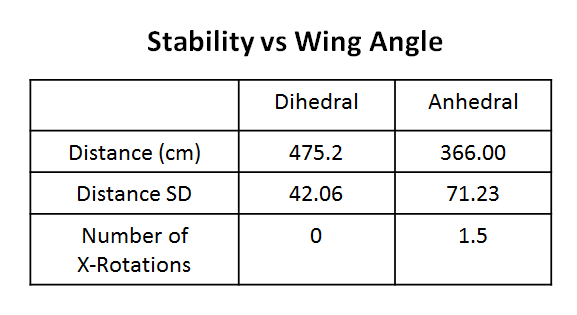
\includegraphics[scale=0.5]{figures/angles.png}
		\caption{Flight distance and stability at different wing angles.}
	\label{fig:angles}
\end{figure}

The data demonstrate that as the wing angle transitions from dihydral to anhydral, the flight becomes shorter and less stable. This supports the prediction in section XXX. 

\subsection{Flight Distance vs Aspect Ratio}

To explore the relation between flight range and aspect ratio, we constructed five The Arrows with different wing span and length. We achieved this by using paper of
different dimension but the same area. As a result, all five paper airplanes have same weight but different aspect ratios. We then launched each of them at the
same height and speed, and recorded the flight distance. To reduce measurement noise, we tested each paper airplane ten times and calculated the average value. See Figure~\ref{fig:aspectratio} 
for the result. 

\begin{figure}[hl]
	\centering
		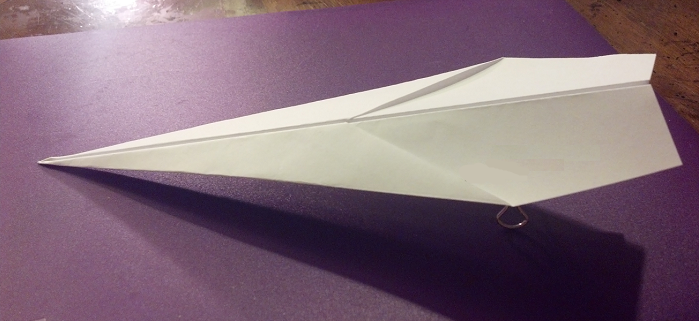
\includegraphics[scale=0.5]{figures/aspectratio.png}
		\caption{The Arrows with different aspect ratios and same weight.}
	\label{fig:aspectratio}
\end{figure}

\begin{figure}[hl]
	\centering
		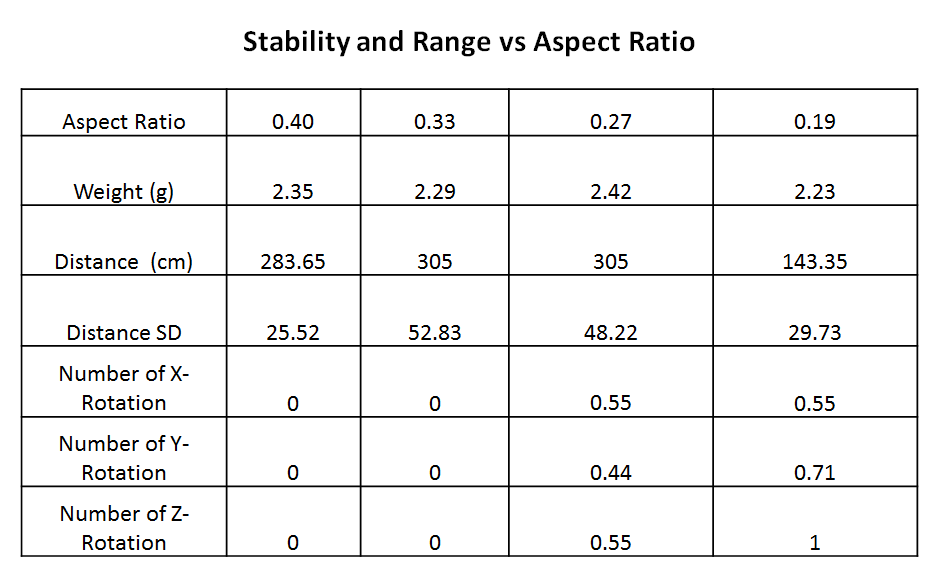
\includegraphics[scale=0.5]{figures/aspectratioresult.png}
		\caption{Flight distance v.s. aspect ratios. The launching height and speed were XXX and XXX, respecitvely. The airplanes weighed XXX g.}
	\label{fig:aspectratioresult}
\end{figure}



The result supports the predictions in section XXX. As aspect ratio increases, the flight becomes XXX and XXX. It's worth noticing that when the aspect ratio is larger than XXX, we observed a flapping motion of the wing. The flight became very unstable and the data were ignored.

\subsection{Drag vs Lift Coefficient}
aa
\subsection{A Comparison of Different Paper Airplane Models}
aa